\documentclass[../main.tex]{subfiles}
%\usepackage{import}
\begin{document}
\section{About this template}
\label{cha:about}

The purpose of this document is two-fold:\\
Firstly, this is a plain and simple template with the most basic \LaTeX-commands and
structures introduced that are
needed for writing a thesis in \LaTeX. It should be sufficient for 95\% of
the theses submitted at LNM - this means that completeness is not claimed. It is recommended to
stick to these basic suggestions, knowing that other - possibly better -
philosophies or styles exist. In case a more complex structure is needed, refer to literature or the web, although you should think
twice about introducing a much more complex structure. \\
Secondly, this report gives some basic suggestions on what the structure of the report should look like and also some brief description about typically expected content.\\

\begin{figure}[h!]
	\begin{center}
	    \includegraphics{\mainpath/fig/tikz/build/setup_quad4_basic_example.pdf}
        %\includestandalone{../fig/tikz/setup_quad4_basic_example}
        %\subimport{../}{/fig/tikz/setup_quad4_basic_example.tex}
        \caption[aaa]{aaa bbb}
		\label{aaa}
    \end{center}
\end{figure}

%\documentclass{standalone}
\usepackage{tikz}
\usetikzlibrary{positioning}
\usetikzlibrary{calc}
\def\mainpath{/home/lukas/Desktop/project/independence/project/thesis/thesis_template}
\def\tikzpath{/home/lukas/Desktop/project/independence/project/thesis/thesis_template/fig/tikz}

\usetikzlibrary{positioning}
\usepackage{pgfplots}
\usepackage{pgfplotstable}
\usepgfplotslibrary{groupplots}



%colors for text highlighting
\definecolor{hlcolor_blue}{RGB}{126,215,255}
\definecolor{hlcolor_green}{RGB}{126,255,175}
\definecolor{hlcolor_orange}{RGB}{246,194,115}
\definecolor{hlcolor_yellow}{RGB}{255,243,113}
\definecolor{hlcolor_purple}{RGB}{215,163,232}

%tikz color list
\definecolor{list1_1}{RGB}{0,101,189}
\definecolor{list1_2}{RGB}{156,157,159}
\definecolor{list1_3}{RGB}{162,173,0}
\definecolor{list1_4}{RGB}{227,114,34} 
\definecolor{list1_5}{RGB}{152,198,234}


%\definecolor{list1_1}{RGB}{246,81,29}
%\definecolor{list1_2}{RGB}{255,180,0}
%\definecolor{list1_3}{RGB}{0,166,237}
%\definecolor{list1_4}{RGB}{127,184,0}
%\definecolor{list1_5}{RGB}{13,44,84}


\pgfplotscreateplotcyclelist{markerlist}{
list1_1, thick, solid, mark=*\\%
list1_2, thick, solid, mark=asterisk\\%
list1_3, thick, solid, mark=diamond*\\%
list1_4, thick, solid, mark=triangle\\%
list1_5, thick, solid, mark=square\\%
}

\pgfplotscreateplotcyclelist{linelist}{
list1_1, solid\\%
list1_2, solid\\%
list1_3, solid\\%
list1_4, solid\\%
list1_5, solid\\%
}

\definecolor{lightgrey}{RGB}{200,200,200}
\definecolor{nassitextcolor}{RGB}{0,0,200}
\begin{document}
\begin{tikzpicture}
		\def\subsize{2}%
		\def\sep{1.0}    %separation between rectangles

	   \def\sep{1.0}    %separation between rectangles       
       %define nodes
       \node (N1) at (-\subsize,-\subsize)  {};%{N1};
       \node (N2) at (0        ,-\subsize)  {};%{N1};
       \node (N3) at (+\subsize,-\subsize)  {};%{N1};
       \node (N4) at (-\subsize,0)          {};%{N1};
       \node (N5) at (0        ,0)          {};%{N1};
       \node (N6) at (+\subsize,0)          {};%{N1};
       \node (N7) at (-\subsize,\subsize)   {};%{N1};
       \node (N8) at (0        ,\subsize)   {};%{N1};
       \node (N9) at (+\subsize,\subsize)   {};%{N1};
       
               % nodes
       \node (N11) at (-\sep-\subsize,+\sep)          {};%{N11};
       
       \node (N12) at (-\sep         ,+\sep)          {};%{N12};
       \node (N13) at (-\sep         ,+\sep+\subsize) {};%{N13};
       \node (N14) at (-\sep-\subsize,+\sep+\subsize) {};%{N14};
       
       \node (N21) at (+\sep         ,+\sep          ){};%{N21};
       \node (N22) at (+\sep+\subsize,+\sep          ){};%{N22};
       \node (N23) at (+\sep+\subsize,+\sep+\subsize) {};%{N23};
       \node (N24) at (+\sep         ,+\sep+\subsize) {};%{N24};
       
       \node (N31) at (+\sep,-\sep-\subsize)          {};%{N31};
       \node (N32) at (+\sep+\subsize,-\sep-\subsize) {};%{N32};
       \node (N33) at (+\sep+\subsize,-\sep)          {};%{N33};
       \node (N34) at (+\sep,-\sep)                   {};%{N34};
       
       \node (N41) at (-\sep-\subsize,-\sep-\subsize) {};%{N41};
       \node (N42) at (-\sep,-\sep-\subsize)          {};%{N42};
       \node (N43) at (-\sep,-\sep)                   {};%{N43};
       \node (N44) at (-\sep-\subsize,-\sep)          {};%{N44};
       
       \draw[fill=lightgrey,thick] (N1) rectangle (N5);
       \draw[fill=lightgrey,thick] (N2) rectangle (N6);
       \draw[fill=lightgrey,thick] (N4) rectangle (N8);
       \draw[fill=lightgrey,thick] (N5) rectangle (N9);
       
       \node[draw, circle, fill=white, font=\small]  at (N1) {1};
       \node[draw, circle, fill=white, font=\small]  at (N2) {2};
       \node[draw, circle, fill=white, font=\small]  at (N3) {3};
       \node[draw, circle, fill=white, font=\small]  at (N4) {4};
       \node[draw, circle, fill=white, font=\small]  at (N5) {5};
       \node[draw, circle, fill=white, font=\small]  at (N6) {6};
       \node[draw, circle, fill=white, font=\small]  at (N7) {7};
       \node[draw, circle, fill=white, font=\small]  at (N8) {8};
       \node[draw, circle, fill=white, font=\small]  at (N9) {9};

		\end{tikzpicture}
		\begin{tikzpicture}
		
		%\definecolor{fillcolor}{RGB}{200,200,200}
       \draw[fill=lightgrey,thick] (N11) rectangle (N13);
       \draw[fill=lightgrey,thick] (N21) rectangle (N23);
       \draw[fill=lightgrey,thick] (N31) rectangle (N33);
       \draw[fill=lightgrey,thick] (N41) rectangle (N43);
       
       %lagrange multipliers
       \draw[<->] (N12) edge (N21) node [fill=white, font=\small] at ($(N12)!0.5!(N21)$) {\framebox{$_2^1$}};
       \draw[<->] (N13) edge (N24) node [fill=white, font=\small] at ($(N13)!0.5!(N24)$) {\framebox{$_4^3$}};
       \draw[<->] (N12) edge (N34) node [fill=white, font=\small] at ($(N12)!0.35!(N34)$) {\framebox{$_6^5$}};
       \draw[<->] (N11) edge (N44) node [fill=white, font=\small] at ($(N11)!0.5!(N44)$) {\framebox{$_8^7$}};
       \draw[<->] (N12) edge (N43) node [fill=white, font=\small] at ($(N12)!0.5!(N43)$) {\framebox{$_{10}^9$}};
       \draw[<->] (N21) edge (N34) node [fill=white, font=\small] at ($(N21)!0.5!(N34)$) {\framebox{$_{12}^{11}$}};
       \draw[<->] (N22) edge (N33) node [fill=white, font=\small] at ($(N22)!0.5!(N33)$) {\framebox{$_{14}^{13}$}};
       \draw[<->] (N21) edge (N43) node [fill=white, font=\small] at ($(N21)!0.35!(N43)$) {\framebox{$_{16}^{15}$}};
       \draw[<->] (N31) edge (N42) node [fill=white, font=\small] at ($(N31)!0.5!(N42)$) {\framebox{$_{18}^{17}$}};   
       \draw[<->] (N34) edge (N43) node [fill=white, font=\small] at ($(N34)!0.5!(N43)$) {\framebox{$_{20}^{19}$}};
       
       
       % doflabels
       \node[anchor=south west]  at (N11) {$_{8}^{7}$};%{N11};
       \node[anchor=south east]  at (N12) {$_{10}^{9}$};%{N12};
       \node[anchor=north east]  at (N13) {$_{16}^{15}$};%{N13};
       \node[anchor=north west]  at (N14) {$_{14}^{13}$};%{N14};
       
       \node[anchor=south west]  at (N21) {$_{10}^{9}$};%{N21};
       \node[anchor=south east]  at (N22) {$_{12}^{11}$};%{N22};
       \node[anchor=north east]  at (N23) {$_{18}^{17}$};%{N23};
       \node[anchor=north west]  at (N24) {$_{15}^{16}$};%{N24};
       
       \node[anchor=south west]  at (N31) {$_{4}^{3}$};%{N31};
       \node[anchor=south east]  at (N32) {$_{6}^{5}$};%{N32};
       \node[anchor=north east]  at (N33) {$_{12}^{11}$};%{N33};
       \node[anchor=north west]  at (N34) {$_{10}^{9}$};%{N34};
       
       \node[anchor=south west]  at (N41) {$_{2}^{1}$};%{N41};
       \node[anchor=south east]  at (N42) {$_{4}^{3}$};%{N42};
       \node[anchor=north east]  at (N43) {$_{10}^{9}$};%{N43};
       \node[anchor=north west]  at (N44) {$_{14}^{13}$};%{N44};
       %\node[circle split, draw, fill=white, font=\small] at (N44) {13 \nodepart{lower} 14};
		
		\end{tikzpicture}
		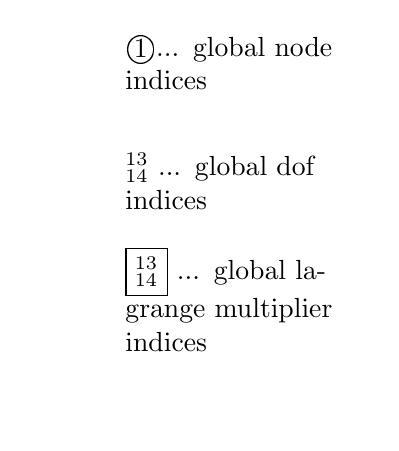
\begin{tikzpicture}
		\node[anchor=south west,text width=3cm] (I1) at (1,0) {\textcircled{\raisebox{-0.9pt}{1}}... global node indices};
		\node [anchor=south west,below of = I1,text width=3cm, node distance=1.5cm] (I2) {$_{14}^{13}$ ... global dof indices};
		\node [anchor=south west,below of = I2,text width=3cm, node distance=1.5cm] (I2) {\framebox{$_{14}^{13}$} ... global lagrange multiplier indices\\};
		\node at (0,-4) {};
		
		\end{tikzpicture}
\end{document}
%\subfile{structure_report}

\textbf{Please note}: 
\begin{itemize}
 \item Significant changes to the document style, layout and structure should only be done according to prior agreement with your supervisor.
 \item compile the template with the following command \\
 \verb|latex LaTeX_template_v04.tex && dvipdfm LaTeX_template_v04.dvi|
 \item if you encounter problems with dvipdfm, you can also use \\
 \verb|latex LaTeX_template_v04.tex && dvi2ps LaTeX_template_v04.dvi &&|\\
 \verb|ps2pdf LaTeX_template_v04.ps| \\
 \item if you use texmaker, or a similar LaTeX editor, declare \verb|LaTeX_template_v04.tex| as master document   \\
 \item the latex compiler might requires 2 or 3 runs, until newly created references are resolved correctly \\
 \item the bibtex file has to be compiled seperately
\end{itemize}

\end{document}